\setcounter{table}{0}
\setcounter{figure}{0}
\renewcommand{\thetable}{A\arabic{table}}
\renewcommand{\thefigure}{A\arabic{figure}}

\section{Desvios do pré-registro}
\label{app:deviations}
% A1: todos os desvios com data (decisions.md). Inclui: inclinação dividida por r, saída em tokens e gaps só dos itens marcados (2026-11-16); confiabilidade na escala 0/1 com termos de projeto (2026-11-14); desvios do Claude: sem seed, temperatura 1,0, Opus sempre pensa, regra over_budget, 2 execuções por orçamento, pesos fechados (2026-11-14); regra de descarte, regra da célula curta não construída, razão pela mediana (2026-11-17); layout só com os passos 1 e 5 (2026-11-17); exclusão dos \excludedDev itens do DevEval cuja referência não passa no corretor (2026-11-25); e os desvios da seção 3.5.
\todo{Tabela A1: todos os desvios com data (tabela escrita à mão)}

\section{Gaps por tamanho}
\label{app:sizes}
% A2: gaps por tamanho e diferenças entre tamanhos (sizes, size_diffs).
\begin{table}[h]
  \centering
  \caption{\todo{legenda da Tabela A2a: gap por tamanho, pp, IC 95\% agrupado}}
  \label{tab:sizes}
  \resizebox{\linewidth}{!}{\begin{tabular}{lccc}
\toprule
Modelo & 10 px & 12 px & 14 px \\
\midrule
\multicolumn{4}{l}{\emph{CoderUJB}} \\
Qwen3.5 27B & \ensuremath{-}33,7 [\ensuremath{-}40,8; \ensuremath{-}26,6] & \ensuremath{-}35,0 [\ensuremath{-}45,3; \ensuremath{-}24,8] & \ensuremath{-}26,2 [\ensuremath{-}35,9; \ensuremath{-}16,5] \\
Gemma 4 12B & \ensuremath{-}35,7 [\ensuremath{-}43,9; \ensuremath{-}27,4] & \ensuremath{-}35,4 [\ensuremath{-}43,0; \ensuremath{-}27,9] & \ensuremath{-}37,6 [\ensuremath{-}46,9; \ensuremath{-}28,4] \\
Mistral Small 3.2 24B & \ensuremath{-}34,7 [\ensuremath{-}45,8; \ensuremath{-}23,5] & \ensuremath{-}30,3 [\ensuremath{-}40,8; \ensuremath{-}19,7] & \ensuremath{-}28,3 [\ensuremath{-}39,4; \ensuremath{-}17,2] \\
Qwen3.5 9B & \ensuremath{-}33,9 [\ensuremath{-}41,2; \ensuremath{-}26,7] & \ensuremath{-}27,3 [\ensuremath{-}31,0; \ensuremath{-}23,6] & \ensuremath{-}25,5 [\ensuremath{-}29,8; \ensuremath{-}21,2] \\
Qwen2.5-VL 7B & \ensuremath{-}14,3 [\ensuremath{-}24,7; \ensuremath{-}4,0] & \ensuremath{-}11,2 [\ensuremath{-}18,3; \ensuremath{-}4,0] & \ensuremath{-}12,9 [\ensuremath{-}21,0; \ensuremath{-}4,7] \\
\midrule
\multicolumn{4}{l}{\emph{DevEval}} \\
Qwen3.5 27B & \ensuremath{-}33,0 [\ensuremath{-}37,8; \ensuremath{-}28,1] & \ensuremath{-}29,0 [\ensuremath{-}33,7; \ensuremath{-}24,3] & \ensuremath{-}22,6 [\ensuremath{-}25,9; \ensuremath{-}19,3] \\
Gemma 4 12B & \ensuremath{-}30,9 [\ensuremath{-}35,5; \ensuremath{-}26,3] & \ensuremath{-}30,6 [\ensuremath{-}36,0; \ensuremath{-}25,3] & \ensuremath{-}30,4 [\ensuremath{-}35,4; \ensuremath{-}25,4] \\
Mistral Small 3.2 24B & \ensuremath{-}33,7 [\ensuremath{-}38,6; \ensuremath{-}28,8] & \ensuremath{-}32,5 [\ensuremath{-}37,3; \ensuremath{-}27,7] & \ensuremath{-}28,3 [\ensuremath{-}32,6; \ensuremath{-}23,9] \\
Qwen3.5 9B & \ensuremath{-}28,4 [\ensuremath{-}33,3; \ensuremath{-}23,5] & \ensuremath{-}23,5 [\ensuremath{-}28,2; \ensuremath{-}18,8] & \ensuremath{-}19,4 [\ensuremath{-}22,9; \ensuremath{-}15,8] \\
Qwen2.5-VL 7B & \ensuremath{-}18,2 [\ensuremath{-}22,5; \ensuremath{-}13,8] & \ensuremath{-}16,5 [\ensuremath{-}20,1; \ensuremath{-}12,9] & \ensuremath{-}14,8 [\ensuremath{-}18,3; \ensuremath{-}11,3] \\
\bottomrule
\end{tabular}
}
\end{table}
\begin{table}[h]
  \centering
  \caption{\todo{legenda da Tabela A2b: diferenças entre tamanhos, pp, IC 95\% agrupado}}
  \label{tab:size-diffs}
  \resizebox{\linewidth}{!}{\begin{tabular}{lccc}
\toprule
Modelo & 12 \ensuremath{-} 10 px & 14 \ensuremath{-} 10 px & 14 \ensuremath{-} 12 px \\
\midrule
\multicolumn{4}{l}{\emph{CoderUJB}} \\
Qwen3.5 27B & \ensuremath{-}1,3 [\ensuremath{-}5,3; 2,6] & 7,5 [4,0; 10,9] & 8,8 [5,2; 12,4] \\
Gemma 4 12B & 0,2 [\ensuremath{-}1,2; 1,7] & \ensuremath{-}2,0 [\ensuremath{-}6,1; 2,2] & \ensuremath{-}2,2 [\ensuremath{-}6,3; 1,8] \\
Mistral Small 3.2 24B & 4,4 [\ensuremath{-}1,2; 10,0] & 6,4 [\ensuremath{-}2,1; 14,8] & 2,0 [\ensuremath{-}4,7; 8,6] \\
Qwen3.5 9B & 6,6 [1,2; 12,0] & 8,5 [0,6; 16,3] & 1,8 [\ensuremath{-}2,9; 6,6] \\
Qwen2.5-VL 7B & 3,2 [\ensuremath{-}3,2; 9,5] & 1,5 [\ensuremath{-}4,9; 7,8] & \ensuremath{-}1,7 [\ensuremath{-}4,7; 1,3] \\
\midrule
\multicolumn{4}{l}{\emph{DevEval}} \\
Qwen3.5 27B & 3,9 [2,4; 5,5] & 10,2 [7,3; 13,2] & 6,3 [3,5; 9,1] \\
Gemma 4 12B & 0,2 [\ensuremath{-}1,5; 1,9] & 0,5 [\ensuremath{-}1,3; 2,2] & 0,3 [\ensuremath{-}1,2; 1,7] \\
Mistral Small 3.2 24B & 1,2 [\ensuremath{-}0,4; 2,7] & 5,3 [3,2; 7,4] & 4,2 [2,4; 5,9] \\
Qwen3.5 9B & 4,9 [3,1; 6,6] & 8,9 [6,3; 11,5] & 4,1 [1,8; 6,3] \\
Qwen2.5-VL 7B & 1,6 [0,0; 3,3] & 3,3 [1,5; 5,1] & 1,7 [\ensuremath{-}0,1; 3,5] \\
\bottomrule
\end{tabular}
}
\end{table}

\section{Correlação da dificuldade entre condições}
\label{app:item-corr}
\begin{figure}[h]
  \centering
  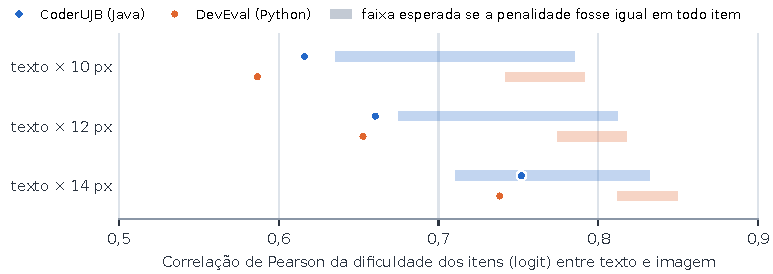
\includegraphics[width=\linewidth]{figures/fig_item_corr}
  \caption{Correlação de Pearson da dificuldade dos itens, em logit, entre texto e cada tamanho de imagem. Os pontos são os valores observados e a faixa clara é o intervalo de 2,5\% a 97,5\% simulado para uma penalidade igual em todo item. Pontos abaixo da faixa indicam que texto e imagem concordam menos do que esse caso prevê.}
  \label{fig:item-corr}
\end{figure}

\section{Análises secundárias do plano}
\label{app:secondary}
% A3: uma linha por análise: comprimento, scoring, lopo (length, scoring, lopo).
\todo{Tabela A3: análises secundárias do plano, uma linha cada}

\section{Claude, exploratório}
\label{app:claude}
% A4: tabela e figura do Claude (claude gaps).
\begin{table}[h]
  \centering
  \caption{\todo{legenda da Tabela A4: Claude, exploratório}}
  \label{tab:claude}
  \resizebox{\linewidth}{!}{\begin{tabular}{lrrcrcr}
\toprule
Modelo & Texto (\%) & Gap (pp) & IC 95\% & Contraste (logit) & IC 95\% & Razão de tokens \\
\midrule
\multicolumn{7}{l}{\emph{CoderUJB, 136 itens}} \\
Claude Sonnet 5.5 & 97,4 & \ensuremath{-}6,2 & [\ensuremath{-}10,8; \ensuremath{-}1,7] & \ensuremath{-}3,08 & [\ensuremath{-}4,88; \ensuremath{-}1,27] & 0,42 \\
Claude Opus 5.5 & 97,4 & \ensuremath{-}2,0 & [\ensuremath{-}3,7; \ensuremath{-}0,3] & \ensuremath{-}1,07 & [\ensuremath{-}2,60; 0,46] & 0,42 \\
\midrule
\multicolumn{7}{l}{\emph{DevEval, 859 itens}} \\
Claude Sonnet 5.5 & 85,4 & \ensuremath{-}6,1 & [\ensuremath{-}8,1; \ensuremath{-}4,2] & \ensuremath{-}1,86 & [\ensuremath{-}2,34; \ensuremath{-}1,39] & 0,42 \\
Claude Opus 5.5 & 92,8 & \ensuremath{-}1,7 & [\ensuremath{-}3,2; \ensuremath{-}0,3] & \ensuremath{-}0,74 & [\ensuremath{-}1,30; \ensuremath{-}0,18] & 0,42 \\
\bottomrule
\end{tabular}
}
\end{table}
\todo{figura do Claude}

\section{Contaminação}
\label{app:contamination}
% A5: tabela de contaminação (contamination.json).
\todo{Tabela A5: contaminação}
